\documentclass[tikz,border=8pt]{standalone}
% Shared look for every TikZ diagram. Load with \input{../../tools/tikz-style.tex}
\usepackage[T1]{fontenc}
\usepackage{lmodern}
\renewcommand{\sfdefault}{lmr}  % diagrams use the same serif as the text
\usetikzlibrary{arrows.meta, positioning, shapes.geometric, calc, fit, backgrounds}
\definecolor{cblue}{HTML}{4C78A8}
\definecolor{corange}{HTML}{F58518}
\definecolor{cgreen}{HTML}{54A24B}
\definecolor{cred}{HTML}{E45756}
\definecolor{cpurple}{HTML}{B279A2}
\definecolor{cgrey}{HTML}{6B6B6B}
\tikzset{
  every picture/.style={font=\sffamily, line width=1.2pt},
  box/.style={draw=#1, fill=#1!12, rounded corners=4pt, align=center, inner sep=7pt, minimum height=1.1cm},
  box/.default=cgrey,
  arrow/.style={-{Stealth[length=3mm]}, draw=cgrey, line width=1.4pt},
  title/.style={font=\sffamily\bfseries\Large},
  note/.style={font=\sffamily\small, text=cgrey, align=center},
}
\AtBeginDocument{\hyphenpenalty=10000 \exhyphenpenalty=10000}

\begin{document}
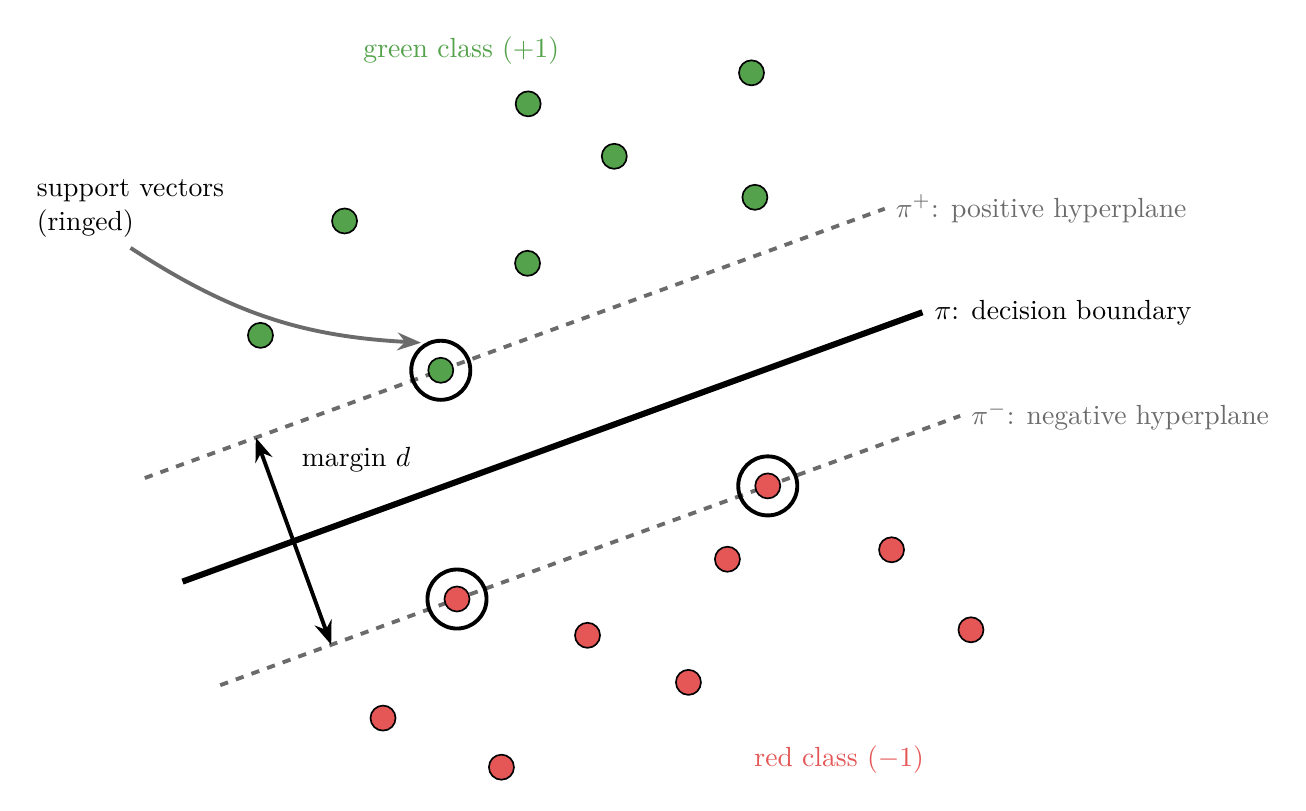
\begin{tikzpicture}[scale=1.0,
  g/.style={circle, fill=cgreen, draw=black, line width=0.6pt, inner sep=3.2pt},
  r/.style={circle, fill=cred, draw=black, line width=0.6pt, inner sep=3.2pt},
  ring/.style={circle, draw=black, line width=1.4pt, minimum size=0.75cm}]
  % hyperplanes (rotated frame: lines are horizontal in a frame turned by 20 degrees)
  \begin{scope}[rotate=20]
    \draw[line width=2.2pt] (-1,0) -- (9,0) node[right] {$\pi$: decision boundary};
    \draw[dashed, cgrey, line width=1.4pt] (-1,1.4) -- (9,1.4) node[right, text=cgrey] {$\pi^{+}$: positive hyperplane};
    \draw[dashed, cgrey, line width=1.4pt] (-1,-1.4) -- (9,-1.4) node[right, text=cgrey] {$\pi^{-}$: negative hyperplane};
    \draw[{Stealth[length=3mm]}-{Stealth[length=3mm]}, line width=1.4pt] (0.5,-1.4) -- (0.5,1.4);
    \node[fill=white, inner sep=2pt] at (1.6,0.7) {margin $d$};
    % support vectors on the dashed lines
    \node[g] (s1) at (3,1.4) {}; \node[ring] at (s1) {};
    \node[r] (s2) at (2.2,-1.4) {}; \node[ring] at (s2) {};
    \node[r] (s3) at (6.4,-1.4) {}; \node[ring] at (s3) {};
    % other points
    \foreach \p in {(1,2.6),(4.5,2.3),(6,3.2),(7.5,2.1),(2.5,3.6),(5.2,4.2),(8,3.6)} \node[g] at \p {};
    \foreach \p in {(0.8,-2.5),(3.6,-2.4),(4.6,-3.4),(7.6,-2.7),(2,-3.6),(5.6,-2.1),(8.2,-4)} \node[r] at \p {};
  \end{scope}
  \node[font=\sffamily, align=left] (sv) at (-1.6,4.4) {support vectors\\(ringed)};
  \draw[arrow] (sv.south) to[bend right=15] ($(20:3) + (110:1.4) + (-0.25,0.35)$);
  \node[font=\sffamily, text=cgreen] at (2.6,6.4) {green class (+1)};
  \node[font=\sffamily, text=cred] at (7.4,-2.6) {red class ($-1$)};
\end{tikzpicture}
\end{document}
